\documentclass[border=0pt]{standalone}
\usepackage[T1]{fontenc}
\usepackage{lmodern,amsmath,graphicx,tikz}
\usetikzlibrary{arrows.meta,calc,positioning}
\definecolor{ink}{HTML}{20252C}
\definecolor{blue}{HTML}{0072B2}
\definecolor{raw}{HTML}{C1272D}
\definecolor{green}{HTML}{39775A}
\definecolor{orange}{HTML}{D55E00}
\definecolor{muted}{HTML}{69717A}
\tikzset{every node/.style={font=\fontsize{9}{10.8}\selectfont,text=ink,inner sep=1mm,outer sep=0pt,align=center},
 title/.style={font=\fontsize{9}{10.8}\selectfont\bfseries},
 detail/.style={font=\fontsize{8.5}{10.2}\selectfont,text=muted},
 box/.style={draw=blue!65,fill=blue!3,line width=.65pt,rounded corners=1mm,minimum height=13mm},
 flow/.style={draw=blue,line width=.8pt,shorten <=.5pt,shorten >=.5pt,-{Latex[length=2mm,width=1.3mm]}},
 ref/.style={draw=green,dashed,line width=.7pt}}

\begin{document}
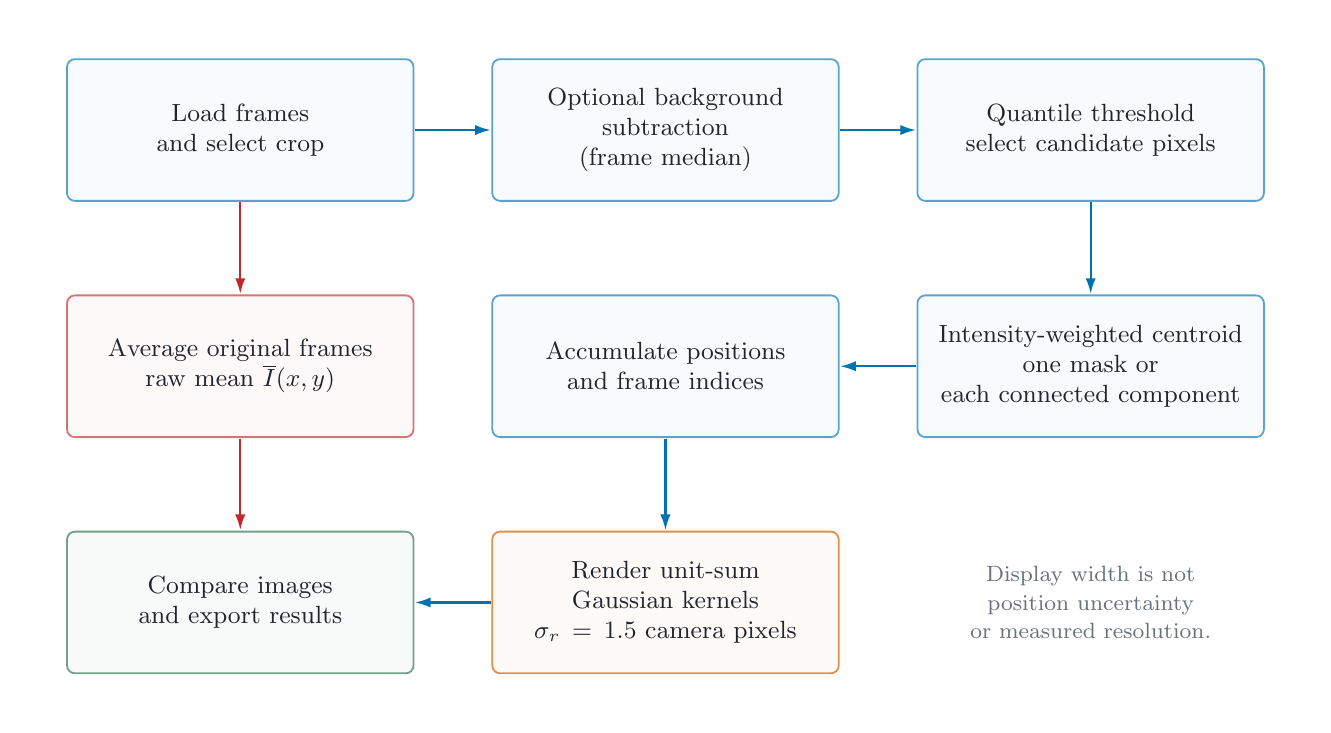
\begin{tikzpicture}[x=1mm,y=1mm,
 stage/.style={box,text width=42mm,minimum height=18mm}]
\path[use as bounding box] (0,0) rectangle (162,86);
% Three aligned columns; each edge terminates at the appropriate box boundary.
\node[stage] (input) at (27,73) {Load frames\\and select crop};
\node[stage] (pre) at (81,73) {Optional background\\subtraction\\(frame median)};
\node[stage] (mask) at (135,73) {Quantile threshold\\select candidate pixels};
\node[stage,draw=raw!65,fill=raw!3] (mean) at (27,43) {Average original frames\\raw mean $\overline I(x,y)$};
\node[stage] (list) at (81,43) {Accumulate positions\\and frame indices};
\node[stage] (loc) at (135,43) {Intensity-weighted centroid\\one mask or\\each connected component};
\node[stage,draw=green!70,fill=green!4] (compare) at (27,13) {Compare images\\and export results};
\node[stage,draw=orange!70,fill=orange!3] (render) at (81,13) {Render unit-sum\\Gaussian kernels\\$\sigma_r=1.5$ camera pixels};
\draw[flow] (input.east)--(pre.west);
\draw[flow] (pre.east)--(mask.west);
\draw[flow] (mask.south)--(loc.north);
\draw[flow] (loc.west)--(list.east);
\draw[flow] (list.south)--(render.north);
\draw[flow] (render.west)--(compare.east);
\draw[flow,draw=raw] (input.south)--(mean.north);
\draw[flow,draw=raw] (mean.south)--(compare.north);
\node[detail,text width=44mm] at (135,13) {Display width is not\\position uncertainty\\or measured resolution.};
\end{tikzpicture}
\end{document}
